\documentclass{standalone}
\usepackage{graphicx}	
\usepackage{amssymb, amsmath}
\usepackage{color}

\usepackage{tikz}
\usetikzlibrary{calc, arrows.meta}
\usepackage{pgfmath}

\definecolor{light}{RGB}{220, 188, 188}
\definecolor{mid}{RGB}{185, 124, 124}
\definecolor{dark}{RGB}{143, 39, 39}
\definecolor{highlight}{RGB}{180, 31, 180}
\definecolor{gray10}{gray}{0.1}
\definecolor{gray20}{gray}{0.2}
\definecolor{gray30}{gray}{0.3}
\definecolor{gray40}{gray}{0.4}
\definecolor{gray60}{gray}{0.6}
\definecolor{gray70}{gray}{0.7}
\definecolor{gray80}{gray}{0.8}
\definecolor{gray90}{gray}{0.9}
\definecolor{gray95}{gray}{0.95}

\newcommand*{\offset}{0.025}

\begin{document}

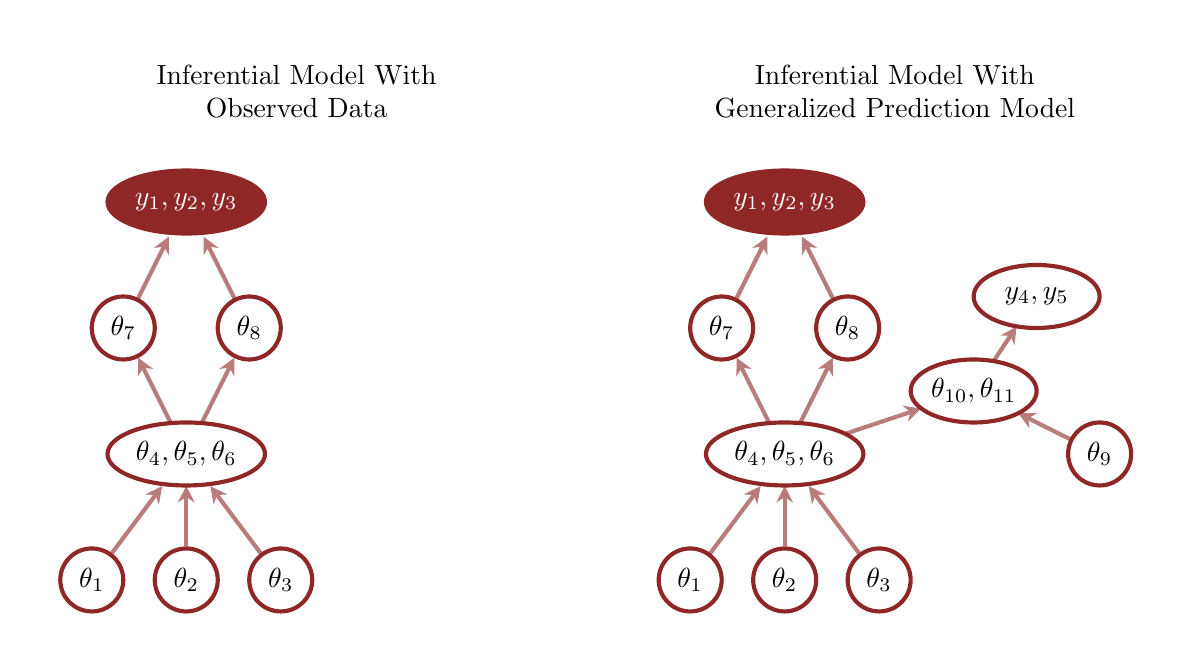
\begin{tikzpicture}[scale=0.2, thick]

  \pgfmathsetmacro{\r}{2}
  
  \begin{scope}[shift={(0, 0)}]
    \draw[white] (-10, -4) rectangle (24, 35);
  
    \node[align=center] at (7, 31) { Inferential Model With\\Observed Data };
  
    \coordinate (A) at (-6, 0);
    \coordinate (B) at (0, 0);
    \coordinate (C) at (+6, 0);
    
    \coordinate (D) at (0, 8);
    
    \coordinate (E) at (-4, 16);
    \coordinate (F) at (+4, 16);
    
    \coordinate (G) at (0, 24);
    
    \coordinate (H) at (20, 8);
    \coordinate (I) at (12, 12);
    \coordinate (J) at (16, 18);
    
    \foreach \B/\E in {D/E, D/F} {
      \draw[-{Stealth[length=6pt, width=6pt]}, shorten <=12.1, shorten >=12, color=mid, line width=1.5] (\B) -- (\E);
    }
    
    \draw[-{Stealth[length=6pt, width=6pt]}, shorten <=12.1, shorten >=14.5, color=mid, line width=1.5] (A) -- (D);
    \draw[-{Stealth[length=6pt, width=6pt]}, shorten <=12.1, shorten >=11.5, color=mid, line width=1.5] (B) -- (D);
    \draw[-{Stealth[length=6pt, width=6pt]}, shorten <=12.1, shorten >=14.5, color=mid, line width=1.5] (C) -- (D);

    \draw[-{Stealth[length=6pt, width=6pt]}, shorten <=12.1, shorten >=14, color=mid, line width=1.5] (E) -- (G);
    \draw[-{Stealth[length=6pt, width=6pt]}, shorten <=12.1, shorten >=14, color=mid, line width=1.5] (F) -- (G);

    \filldraw[fill=white, draw=dark, line width=1.5] (A) circle (\r)
    node[color=black] { $\theta_{1}$ };

    \filldraw[fill=white, draw=dark, line width=1.5] (B) circle (\r)
    node[color=black] { $\theta_{2}$ };

    \filldraw[fill=white, draw=dark, line width=1.5] (C) circle (\r)
    node[color=black] { $\theta_{3}$ };
    
    \filldraw[fill=white, draw=dark, line width=1.5] (D) circle [x radius={2.5 * \r}, y radius={\r}]
    node[color=black] { $\theta_{4}, \theta_{5}, \theta_{6}$ };
    
    \filldraw[fill=white, draw=dark, line width=1.5] (E) circle (\r) 
    node[color=black] { $\theta_{7}$ };
    
    \filldraw[fill=white, draw=dark, line width=1.5] (F) circle (\r)
    node[color=black] { $\theta_{8}$ };
      
    \filldraw[fill=dark, draw=dark, line width=1.5] (G) circle [x radius={2.5 * \r}, y radius={\r}]
    node[color=white] { $y_{1}, y_{2}, y_{3}$ };

  \end{scope}

  \begin{scope}[shift={(38, 0)}]
    \draw[white] (-10, -4) rectangle (24, 35);
  
    \node[align=center] at (7, 31) { Inferential Model With\\Generalized Prediction Model };
  
    \coordinate (A) at (-6, 0);
    \coordinate (B) at (0, 0);
    \coordinate (C) at (+6, 0);
    
    \coordinate (D) at (0, 8);
    
    \coordinate (E) at (-4, 16);
    \coordinate (F) at (+4, 16);
    
    \coordinate (G) at (0, 24);
    
    \coordinate (H) at (20, 8);
    \coordinate (I) at (12, 12);
    \coordinate (J) at (16, 18);
    
    \foreach \B/\E in {D/E, D/F} {
      \draw[-{Stealth[length=6pt, width=6pt]}, shorten <=12.1, shorten >=12, color=mid, line width=1.5] (\B) -- (\E);
    }
    
    \draw[-{Stealth[length=6pt, width=6pt]}, shorten <=12.1, shorten >=14.5, color=mid, line width=1.5] (A) -- (D);
    \draw[-{Stealth[length=6pt, width=6pt]}, shorten <=12.1, shorten >=11.5, color=mid, line width=1.5] (B) -- (D);
    \draw[-{Stealth[length=6pt, width=6pt]}, shorten <=12.1, shorten >=14.5, color=mid, line width=1.5] (C) -- (D);

    \draw[-{Stealth[length=6pt, width=6pt]}, shorten <=12.1, shorten >=14, color=mid, line width=1.5] (E) -- (G);
    \draw[-{Stealth[length=6pt, width=6pt]}, shorten <=12.1, shorten >=14, color=mid, line width=1.5] (F) -- (G);

    \draw[-{Stealth[length=6pt, width=6pt]}, shorten <=12.1, shorten >=20, color=mid, line width=1.5] (D) -- (I);
    \draw[-{Stealth[length=6pt, width=6pt]}, shorten <=12.1, shorten >=18, color=mid, line width=1.5] (H) -- (I);
    \draw[-{Stealth[length=6pt, width=6pt]}, shorten <=12.1, shorten >=13, color=mid, line width=1.5] (I) -- (J);

    \filldraw[fill=white, draw=dark, line width=1.5] (A) circle (\r)
    node[color=black] { $\theta_{1}$ };

    \filldraw[fill=white, draw=dark, line width=1.5] (B) circle (\r)
    node[color=black] { $\theta_{2}$ };

    \filldraw[fill=white, draw=dark, line width=1.5] (C) circle (\r)
    node[color=black] { $\theta_{3}$ };
    
    \filldraw[fill=white, draw=dark, line width=1.5] (D) circle [x radius={2.5 * \r}, y radius={\r}]
    node[color=black] { $\theta_{4}, \theta_{5}, \theta_{6}$ };
    
    \filldraw[fill=white, draw=dark, line width=1.5] (E) circle (\r) 
    node[color=black] { $\theta_{7}$ };
    
    \filldraw[fill=white, draw=dark, line width=1.5] (F) circle (\r)
    node[color=black] { $\theta_{8}$ };
      
    \filldraw[fill=dark, draw=dark, line width=1.5] (G) circle [x radius={2.5 * \r}, y radius={\r}]
    node[color=white] { $y_{1}, y_{2}, y_{3}$ };

    \filldraw[fill=white, draw=dark, line width=1.5] (H) circle (\r)
    node[color=black] { $\theta_{9}$ };
    
    \filldraw[fill=white, draw=dark, line width=1.5] (I) circle [x radius={2 * \r}, y radius={\r}]
    node[color=black] { $\theta_{10}, \theta_{11}$ };
    
    \filldraw[fill=white, draw=dark, line width=1.5] (J) circle [x radius={2 * \r}, y radius={\r}]
    node[color=black] { $y_{4}, y_{5}$ };

  \end{scope}

\end{tikzpicture}

\end{document}  